\chapter{Metodologia}

O objetivo geral deste trabalho é realizar uma análise da API do sistema Android a partir de uma análise estática de seu código fonte, e então avaliar a possibilidade de utilizar os resultados como referência para o desenvolvimento de aplicativos desenvolvidos para o Android, partindo da premissa que os aplicativos desenvolvidos utilizando a API do sistema são fortemente dependentes da mesma. (citar fontes)

A partir da análise do código fonte, traçar um perfil que caracteriza o próprio sistema a partir de suas métricas de código fonte, assim como traçar esse perfil para os aplicativos do sistema e verificar o grau de aproximação que ambos encontram em seu design. 

Assumindo que o código dos aplicativos do sistema possuem a arquitetura ideal de aplicativos por serem mantidos pela Google, bem como pela comunidade de desenvolvedores por ter código aberto, criar então um fator de aproximação para aplicar em aplicativos em desenvolvimento para avaliar sua qualidade de acordo com a aproximação ao sistema e à aplicativos nativos, em termos de métricas estáticas de código. Esse fator de aproximação pode ser calculado utilizando métodos estatísticos ou aprendizado de máquina, de forma que possa ser avaliada a aproximação de uma nova amostra aos perfis existentes.

Caso o grau de aproximação de um aplicativo qualquer seja bastante elevado, pode-se inferir uma boa qualidade de código, pelo fato de se aproximar àquelas desenvolvidas pelos próprios arquitetos do sistema.

Utilizar para isso métricas de código orientado a objeto, bem como outras métricas que refletem decisões arquiteturais e de design. É importante incluir métricas que refletem o volume de código para dar resultados relativos ao tamanho do aplicativo sendo avaliado, uma vez que várias métricas tem seu valor de referência variável de acordo com o tamanho do código. Utilizar valores do sistema, como milhões de linhas de código, como referencia para analisar um aplicativo com apenas algumas centenas de linhas resulta em uma comparação inválida para os valores de algumas métricas.

Algumas conclusões talvez já possam ser tiradas de acordo com a aproximação do código do sistema aos aplicativos nativos, caso os mesmos sejam a referencia. Por exemplo, a respeito dos aplicativos nativos, se os resultados mostrarem que nenhum se aproxima a mais de 70\% do sistema, então pode-se inferir que a aproximação ideal ao sistema seja esta, e talvez uma maior que 70 não seja desejada em aplicativos de terceiros. Da mesma forma, uma aproximação muito alta pode indicar a possibilidade de utilizar os valores da mesma como referência, utilizando os aplicativos para gerar mais amostras relativas de tamanho.

\section{Pesquisa}

Baseando-se as ideias apresentadas, são levantadas as seguintes questões de pesquisa:

\begin{itemize}
\item É possível monitorar métricas estáticas de código fonte de aplicativos Android de acordo com a análise e predição da evolução do código do sistema?
\item É efetivo usar o próprio sistema como arquitetura referencia devido ao acoplamento de aplicativos com a própria API de desenvolvimento?
\end{itemize}

Para alcançar os objetivos descritos e responder as questões de pesquisa que foram definidas, algumas hipóteses devem ser estudadas e avaliadas:

\begin{itemize}
\item É possível identificar padrões e tendências na evolução da arquitetura do sistema Android e nos aplicativos desenvolvidos para ele.
\item O desenvolvimento de aplicativos Android pode ser guiado pelo resultado de uma análise evolutiva do código do próprio sistema.
\end{itemize}

Como uma hipótese adicional neste trabalho, será avaliado o resultado do trabalho anterior em desenvolvimento de uma arquitetura Android em contraste com este estudo. Em trabalho anterior (referenciar), foram tomadas diversas decisões teóricas com o objetivo de alcançar a melhor arquitetura para um aplicativo Android desenvolvido para um estudo de caso específico. Surge então uma hipótese adicional, para avaliar se as decisões tomadas com base em experiência de desenvolvedor e padrões de projeto são refletidas e semelhantes as decisões que podem ser tomadas com base em resultados de análise estática de código fonte, como as análises realizadas neste trabalho.

\begin{itemize}
\item As decisões arquiteturais teóricas aplicadas no estudo de caso biodyn estão relacionadas com decisões arquiteturais baseadas em métricas.
\end{itemize}

O projeto do aplicativo desenvolvido nesse estudo de caso específico também deve ser submetido a análise de aproximação ao código do sistema e de aplicativos nativos, de forma a validar as decisões tomadas durante o desenvolvimento do mesmo.

Como uma última hipótese adicional, pode ser testada afirmação a seguir, esperando que as demais análises já tragam informações relevantes por consequência dos suas próprios resultados.

\begin{itemize}
\item É possível traçar um perfil de design para um desenvolvedor, ou equipe de desenvolvimento, e assim detectar aplicativos de sua autoria.
\end{itemize}

Essa hipótese se dá pelo fato de que cada equipe tem uma espécie de estilo de arquitetura ou estilo de codificação, que pode estar refletido nas métricas estáticas de código fonte de seus projetos.

\section{Trabalhos relacionados}

\citeonline{androidblackberry}  realiza um estudo de dependência das APIs de desenvolvimento tanto da plataforma Android quanto da plataforma Blackberry, a fim de fazer uma comparação entre os sistemas. A partir disso, é verificado o quanto uma API influencia na quantidade de código desenvolvido, assim como é verificada a dependência de código de terceiros para o desenvolvimento de aplicativos. Em suma, o resultado comparativo demonstrou que aplicativos no sistema Android são significativamente mais dependentes da API do sistema devido a maior completude da API, reduzindo por consequência a quantidade de código de terceiros e código próprio dentro dos projetos. Embora possa tornar mais fácil o desenvolvimento, essa dependência maior em relação ao código do sistema torna o código de aplicativo desenvolvido para Android difícil de ser portado para outras plataformas.

\citeonline{samoa} apresenta o desenvolvimento de uma ferramenta de análise estática de código, que avalia não apenas métricas de código fonte do sistema, como dependência de código de terceiros dentro do projeto de aplicativos Android. O objetivo não é apenas analisar software em plataforma móvel, mas também diferenciar a abordagem quado analisando um software tradicional ou um software para dispositivo móvel, de forma a verificar a manutenibilidade desses sistemas. O estudo de \citeonline{androidblackberry} também apresenta algumas discussões no quesito manutenibilidade em sistemas móveis. Assim como neste último, \citeonline{samoa} demonstra uma alta dependência de aplicativos android em relação ao sistema, apresentando em geral cerca de  2/3 das chamadas de método de aplicativos sendo para bibliotecas externas ao app, em sua maioria para a API Android ou métodos de bibliotecas padrão java.

\citeonline{evolutionandroid} reforça a idéia de dependência de aplicativos em relação a API Android, e fala um pouco sobre as grandes mudanças da API devido a sua rápida evolução nos ultimo anos. Tenta então ajudar desenvolvedores com dicas para melhor se prepararem para mudanças na plataforma, assim como para mudanças em bibliotecas de terceiros, que podem ser bastante significativas em diversos aspectos, e consequentemente impactar negativamente no desenvolvimento de aplicativos, introduzindo mudanças bruscas e possivelmente bugs.

A dependência dos aplicativos Android em relação ao próprio sistema fica bem clara em vários trabalhos publicados até a data de escrita deste trabalho, o que motiva bastante a coleta e análise de métricas no sistema para serem comparadas com métricas de aplicativos. Os resultados podem ser bastante úteis para novos desenvolvedores que não têm referências para basear seu desenvolvimento e poderiam guiar a evolução de seu sistema em comparação com a evolução do próprio Android.

Em se tratando de métricas, \citeonline{predictivemodels} apresenta várias abordagens para analisar métricas em software, mais a nível de projeto, e gerar modelos preditivos. Vários métodos de aprendizado de máquina são explanados e comparados em termos de modelagem relacionada a métricas em software. 

\citeonline{qualitypredictionsvm} apresenta um método utilizando support vector machine, um modelo na área de machine learning, para prever qualidade de software em estágios iniciais de desenvolvimento baseado em métricas de complexidade de código, usando quantidade de linhas de código e outras métricas como métricas de complexidade de Halstead e complexidade ciclomática.

\citeonline{evaluatingpredictivemodels} descreve uma comparação de várias técnicas para prever qualidade de código, classificando como alto risco, com grande probabilidade de conter erros, ou baixo risco, com probabilidade de conter poucos ou nenhum erro. vários métodos são avaliados desde regressão linear até redes neurais. Embora os resultados apresentados no artigo não tenham sido muito promissores, algumas observações podem ser tiradas como exemplo para trabalhos relacionados. Neste trabalho, por exemplo, a qualidade de código será avaliada não pela probabilidade de conter falhas como nesse artigo, mas sim em um estudo de correlação entre um projeto em análise com os códigos nativos do sistema, onde se espera ter a arquitetura ideal projetada para a plataforma alvo. 

Ainda tentando avaliar a probabilidade de conter erros, \citeonline{validationmetricsfaultprediction} também utiliza técnicas de machine learning, utilizando como dados essencialmente métricas orientadas a objeto de Chidamber e Kemerer. Esse estudo é conduzido em cima de software livre, utilizando como estudo de caso o Mozilla. Uma das contribuições que o artigo apresenta é relacionar classes e bugs reportados dentro do Mozilla. Além disso, verificaram que a métrica de acoplamento entre objetos (\textit{coupling between objects} - CBO) foi a mais determinante em prever probabilidade de falha em classes, refletindo um pouco da qualidade do código escrito. Da mesma forma, a métrica linhas de código (\textit{lines of code} - LOC) tabém se mostrou bastante útil, assim como a métrica de falta de coesão em métodos (\textit{Lack of Coesion On Methods} - LCOM). Outras observações são que as métricas de profundidade de herança (\textit{Depth In Tree} - DIT) se mostrou não muito deterministica, ao mesmo tempo que  número de classes também não teve impacto nos resultados. É importante notar que essas observações são válidas para o Mozilla, escrito em C/C++, o que não implica necessariamente que sejam válidas para todas as linguagens, embora isso seja bastante provável.

Existem vários outros trabalhos publicados a respeito de prevenção de falhas com verificação da qualidade do código fonte, porém a principal diferenciação deste trabalho em relação a eles é o fato de a qualidade não ser medida em quantidade de bugs/erros ou modificações do código, mas sim como o resultado de uma comparação do código com a arquitetura do sistema e de aplicativos nativos, considerada ideal por ser desenvolvida pela mesma empresa criadora e mantenedora do sistema operacional. Entretanto, os dados utilizados neste trabalho serão essencialmente os mesmos da maioria desses trabalhos, resumindo-se basicamente em métricas OO de Chidamber e Kemerer, métricas de complexidade e de volume de código fonte.

\section{Coleta de Dados}

O código fonte para análise foi retirado diretamente do \textit{Android Open Source Project}\footnote{\url{http://source.android.com/}}  (AOSP). Esse código é mantido essencialmente pela Google, com colaboração da comunidade de desenvolvedores. Essa versão é mantida e evoluída para funcionar como base para que as fabricantes de dispositivos possam manter sempre a ultima versão do sistema, com atualizações funcionais e de segurança, enquanto trabalham em ideias inovadoras para melhorar a experiência de usuário de seus dispositivos. A Motorola, por exemplo, tem o seu sistema levemente modificado para incluir algumas funcionalidades em seus produtos, assim como várias outras grandes fabricantes como a Samsung, LG e outras.  Essa forma de manter o sistema aberto e altamente customizável mantém uma competitividade entre as empresas, pois partindo do mesmo sistema base, todas as fabricantes entregam a seus clientes dispositivos com essencialmente as mesmas funcionalidades, com exceção das pequenas modificações, em um sistema operacional robusto e estável.

A ferramenta \textit{repo} é utilizada para unificar os projetos internos dos componentes do sistema em seus repositórios, e um tutorial para configurar a ferramenta e fazer o download do projeto pode ser encontrado no site do AOSP.

Para a análise da API do sistema, foram escolhidas 16 versões do sistema, selecionando arbitrariamente a primeira e a última versão de cada grande \textit{release}. Por exemplo, para o \textit{Android Eclair}, foram pegas as versões 2.0 e 2.1, e para o KitKat, as versões 4.4 e 4.4.4. Para o \textit{Android Lollipop}, a última versão selecionada não será a ultima antes da próxima grande \textit{release}, mas sim a última lançada até a data de início deste trabalho. Em uma análise ideal, todas as versões possíveis seriam levadas em consideração, mas o motivo dessa escolha de versões foi a impossibilidade de realizar uma análise do código fonte de todas as versões para este trabalho, por limitações de tempo e de recursos computacionais. Portanto, foram escolhidas as versões iniciais de cada grande \textit{release} onde é alterado o \textit{codename} da versão, que contém grandes mudanças e significativos avanços no sistema, assim como as versões finais de cada \textit{codename}, que representam as versões mais estáveis das funcionalidades adicionadas nas versões com aquele \textit{codename}.
 
Cada versão escolhida corresponde a uma \textit{TAG} no repositório oficial. Segue a listagem das \textit{tags} escolhidas:
\begin{enumerate}
\item \textit{Android Donut} 1.6 r1.2
\item \textit{Android Donut} 1.6 r1.5
\item \textit{Android Eclair} 2.0 r1
\item \textit{Android Eclair} 2.1 r2.1p2
\item \textit{Android Froyo} 2.2 r1
\item \textit{Android Froyo} 2.2.3 r2
\item \textit{Android Gingerbread} 2.3 r1
\item \textit{Android Gingerbread} 2.3.7 r1
\item \textit{Android Ice Cream Sandwich} 4.0.1 r1
\item \textit{Android Ice Cream Sandwich} 4.0.4 r2.1
\item \textit{Android Jelly Bean} 4.1.1 r1
\item \textit{Android Jelly Bean} 4.3.1 r1
\item \textit{Android KitKat} 4.4 r1
\item \textit{Android KitKat} 4.4.4 r2
\item \textit{Android Lollipop} 5.0.0 r1.0.1
\item \textit{Android Lollipop} 5.1.0 r1
\end{enumerate}

\begin{figure}[!htb]
\centering
\includegraphics [keepaspectratio=true,scale=0.35]{figuras/androidSourceFolders.eps}
\caption{Exemplo de estrutura de arquivos de diretório raiz do AOSP}
\label{androidSourceFolders}
\end{figure}

Para cada \textit{tag}, foi criado um diretório separado em um sistema Debian, onde foi executada o comando "repo -init" com um complemento específico para \textit{setup} inicial daquela \textit{tag}. Esse comando prepara o diretório e cria arquivos de controle da ferramenta para o repositório que está sendo iniciado. São baixados alguns arquivos, como por exemplo o arquivo em xml, chamado \textit{manifest}, que contém os projetos ou repositórios que compõe o sistema, todos para a tag específica que foi iniciada. Antes de fazer o download do código, foram retirados do \textit{manifest} da ferramenta todos os subprojetos que não estavam contidos dentro da pasta \textit{frameworks}, que é o principal alvo da análise. Desas forma só os projetos de interesse são baixados quando o download for feito. Essa escolha se deu pelo fato de que grande parte do código java da API do sistema utilizado no desenvolvimento de aplicativos se encontra neste local. Cyanogenmod, uma das maiores e mais conhecidas versões alternativas ao AOSP mas ainda baseada no mesmo, mantida por colaboradores voluntários em paralelo ao código da Google, citam em sua página de ajuda a desenvolvedores\footnote{\url{http://wiki.cyanogenmod.org/w/Doc:_the_cm_source}}  que o diretório \textit{frameworks} é onde se encontram os "\textit{hooks}" que programadores usam para construir seus aplicativos, ou seja, a API de construção de aplicativos em geral. O restante dos diretórios do AOSP contém desde adaptações de bibliotecas para o Android como o bionic, até código fonte para o \textit{Android Run Time} (ART), que substituiu a dalvik nas ultimas versões do sistema (especificamente desde as versões de \textit{codename Lollipop}), e também códigos de baixo nível específicos para alguns dispositivos. Também existem diretórios para projetos externos ao Android, utilizados pelo mesmo, como o SQLite e outros projetos externos. O kernel utilizado no sistema também tem o seu diretório nessa hierarquia, assim como os aplicativos nativos. A estrutura completa do AOSP não será explorada neste trabalho, mas o conteúdo da pasta raiz pode ser visualizado na figura \ref{androidSourceFolders}.

\begin{figure}[!htb]
\centering
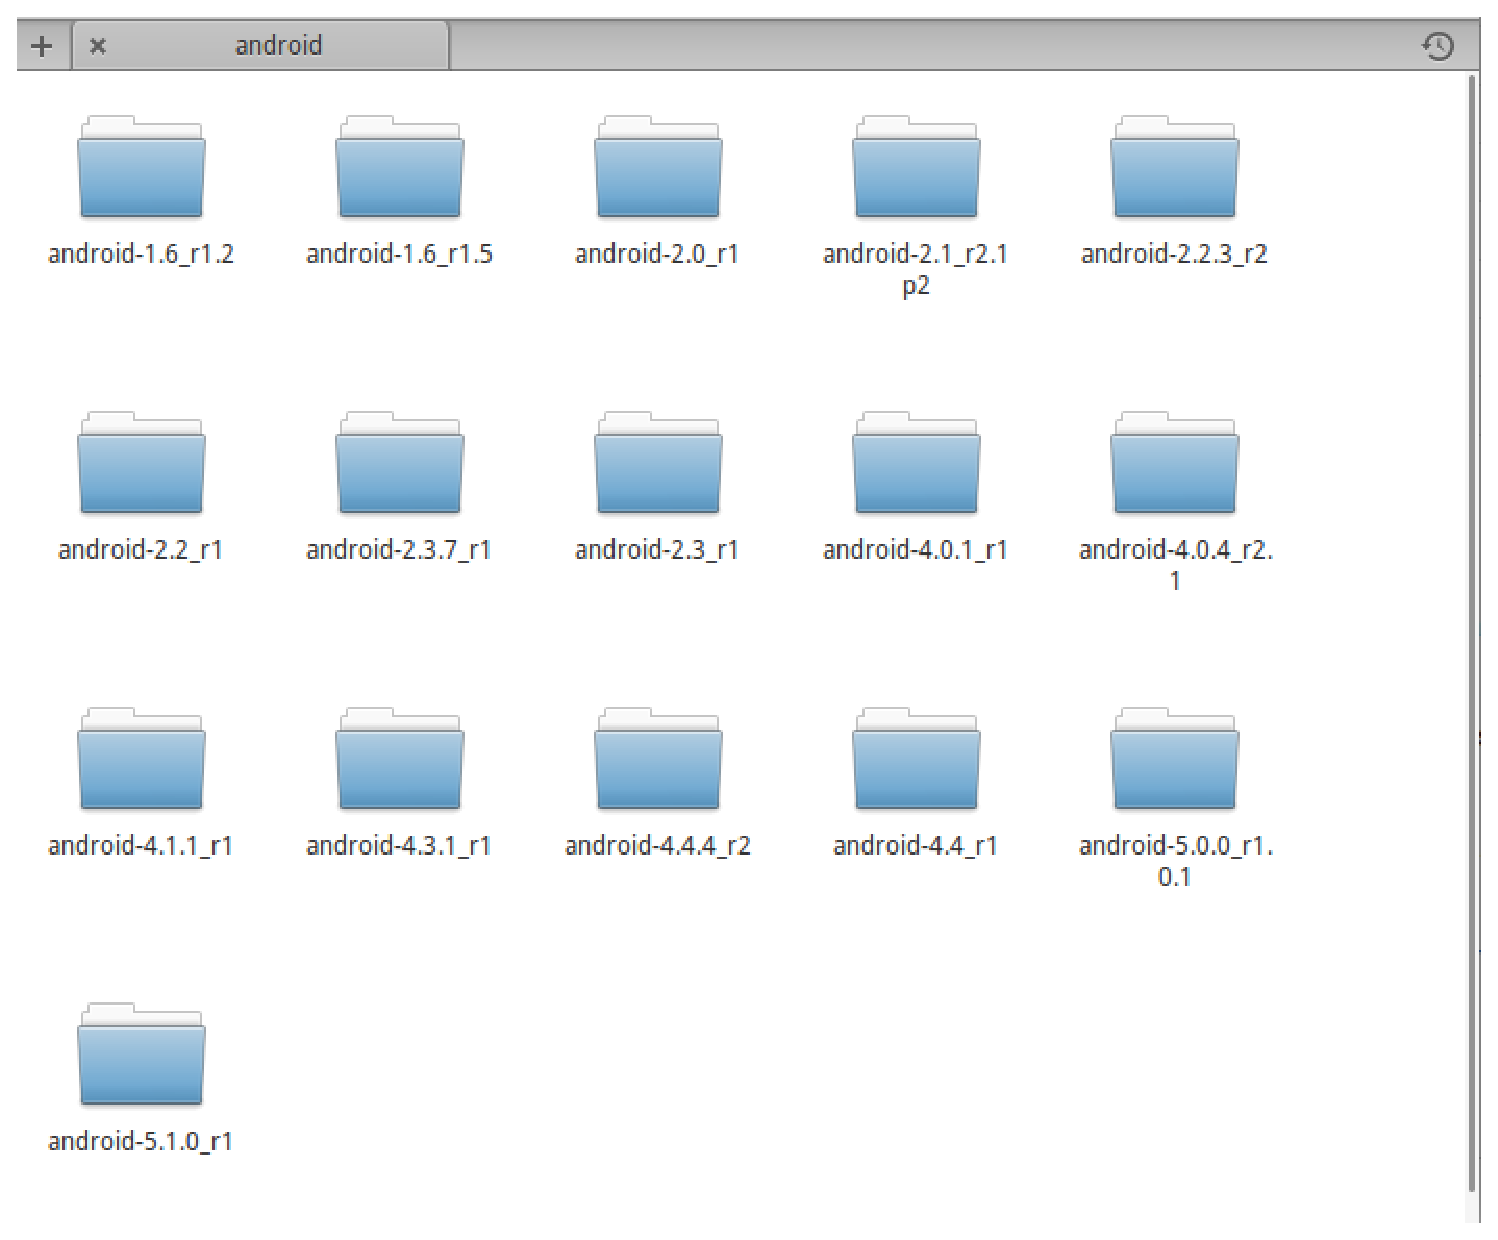
\includegraphics [keepaspectratio=true,scale=0.35]{figuras/folder.eps}
\caption{Diretório onde foram armazenadas cada versão a ser analisada}
\label{folder}
\end{figure}

A estrutura de diretórios onde foram preparados os códigos para a análise pode ser vista na figura \ref{folder}.

Em seguida foi feito o download de cada \textit{tag} em seu diretório, também utilizando a ferramenta \textit{repo}, que realiza um \textit{checkout} de cada subprojeto listado em seu \textit{manifest} através do comando \textit{sync}. O total de espaço em disco ocupado após o download de todas as \textit{TAGS} foi cerca de 10 GB. É importante notar que boa parte deste espaço corresponde a arquivos de mídia ou outros formatos que fazem parte do sistema mas não serão analisados por não corresponderem a código fonte. Não foi realizado nenhum tipo de filtro para remover esses arquivos nem antes nem durante a análise estática de código, porém isso afeta apenas a performance da ferramenta de análise, mas os resultados permanecem sem interferência.

Após o download de todas as versões escolhidas, foi utilizada a ferramenta Analizo\footnote{\url{http://www.analizo.org/}}  para análise estática de código e coleta de métricas. Um dos motivos da escolha do sistema Debian foi a facilidade de instalação da ferramenta. O Analizo é uma ferramenta livre e extensível para análise de código com suporte a várias linguagens, incluindo java, que será o foco da análise neste trabalho. Uma grande quantidade de métricas são coletadas pela ferramenta, embora apenas algumas sejam utilizadas para  esta análise. Foram coletadas essencialmente métricas de código fonte orientado a objetos. São métricas desse tipo que melhor refletem as decisões arquiteturais ou de design aplicadas durante o desenvolvimento do sistema.

Neste trabalho, foi utilizada a funcionalidade de \textit{batch} do Analizo, de forma a coletar métricas de todas as \textit{tags} de uma só vez. A saída da ferramenta é um arquivo CSV para cada projeto ou versão a ser analisada, assim como um arquivo CSV que centraliza os valores de cada métrica a nível de projeto para cada um dos projetos/versões. Isso pode ser interessante quanto utilizado com o mesmo projeto em diferentes versões para verificar o avanço de algumas métricas juntamente com a evolução do sistema.